\documentclass[a4wide]{report}
\usepackage{amsmath}
\usepackage[a4paper, total={7in, 10.2in}]{geometry}
\usepackage{graphicx}
\usepackage[portuguese]{babel}
\usepackage[utf8]{inputenc}
\usepackage{sidecap}
\usepackage{subfigure}

\begin{document}

\noindent
{\bf Lincoln Martins de Oliveira (ES 90693) - Mini-relatório 04 (\today)}

\begin{quote}

\centering

\bf Mini relatório referente ao exercício 1 e 2 das aulas 21 e 22

\end{quote}
\vspace{0.5cm}
\begin{quote}

\bf  Exercício 1:

\end{quote}

Neste exercício nos considerei uma partícula submetida ao potencial Morse $U(r) = -D (1 - [1 - exp(-a(r - r_{e}))^{2}])$ onde nos foi dado
os valores D = 1, a = 1, $r_{e} = 0$ , e = -0.8 , m = 1 e com isso fui capaz de encontrar a força : $F(r) = \frac{-dU }{dr}(r) = -2e^{-r} (1 - e^{-r} )$ .
Sabe-se que $\frac{F}{m} = a$, como m = 1 encontrei deste modo a aceleração da partícula dada por \ref{fun1}.

\begin{equation}
\centering
a = -2e^{-r} (1 - e^{-r} )
\label{fun1}
\end{equation}

\begin{quote}

\bf a-

\end{quote}

 Nessa primeira alternativa o objetivo foi utilizar os métodos de verlet original, e velocity verlet para resolver equações 
 diferenciais de segunda ordem, e a partir da aceleração obter as velocidades e posições em função do tempo de uma partícula. Eu utilizei dois programas 
 para resolver toda a questão 1, alternativas a e b, cujos nomes são $''ex01a.f90''$ e $''ex01a_Runge-kutta.f90''$ e estao na pasta ex01. Os resultados serão 
 mostrados abaixo. 
 
 A figura \ref{gra1} mostra os resultados para os valores de posição da partícula r(t) encontrados utilizando os métodos de Verlet original,
 velocity Verlet e Runge Kutta. O gráfico \ref{gra2} mostra os resultados para os valores das velocidades da partícula v(t) encontradas utilizando os três métodos.
 Podemos notar que para qualquer um dos métodos foram encontrados valores próximos de posição e velocidade para a partícula como pode ser visto nos gráficos \ref{gra1} e \ref{gra2}.

 
\begin{figure}[!ht]
\centering
\includegraphics[width=0.80\textwidth]{ex011.eps}
\caption{Gráfico comparando as posições da partícula para os métodos de verlet original, velocit verlet e Runge Kutta.}
\label{gra1}
\end{figure}

\newpage

\begin{figure}[!ht]
\centering
\includegraphics[width=0.70\textwidth]{ex012.eps}
\caption{Gráfico comparando as velocidades da partícula para os métodos de verlet original, velocit verlet e Runge-Kutta.}
\label{gra2}
\end{figure}



Sabendo-se que a solução exata do $\bf PVI$ é dada por \ref{fun2}, já que esta nos foi dada pela referência \cite{FL}, podemos comparar então
a solução exata com os métodos computacionais utilizados aqui para se obter a posição r(t) da partícula e ver o quão preciso são tais ferramentas.

\begin{equation}
\centering
r(t) = r_0 + a^{-1} ln[s(t)]
\label{fun2}
\end{equation}

onde,

\begin{equation}
\centering
s(t) = \frac{(-1 + \sqrt{e + 1} cos(\sqrt{-2e}t - acos(\sqrt{e + 1}))}{e}
\label{fun3}
\end{equation}

Na figura \ref{gra3} compara-se respectivamente as posições da partícula r(t) obtidas pelos métodos de verlet original, velocity verlet e Runge Kutta com a solição exata.
Pode-se notar que as posições obtidas por estes métodos se sobrepõem.


\begin{figure}[!ht]
\centering
\subfigure[Gráfico de Verlet original versus solução exata.]{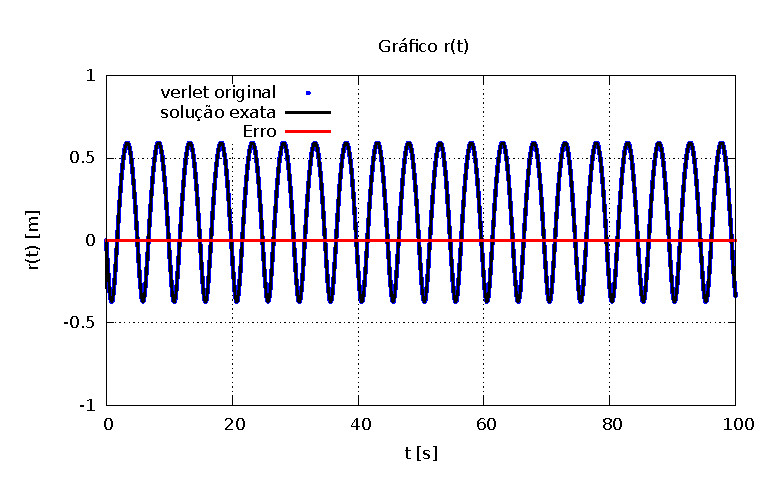
\includegraphics[scale=0.55]{ex013.eps}}\qquad 
\subfigure[Gráfico de velocity Verlet versus solução exata.]{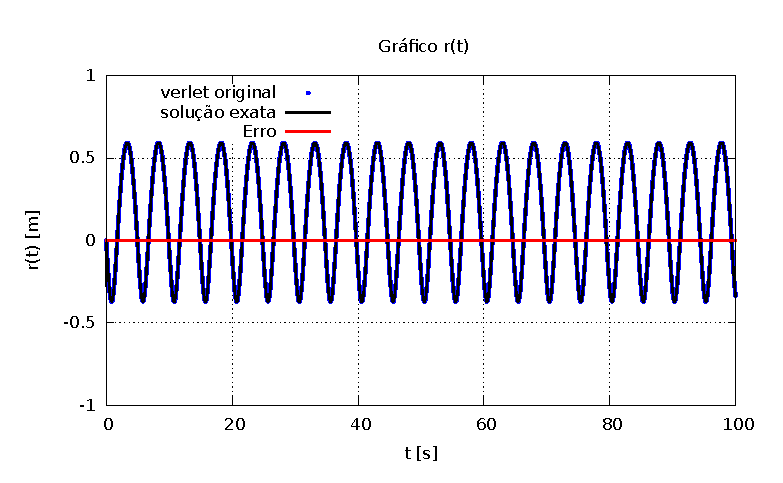
\includegraphics[scale=0.55]{ex014.eps}}\qquad 
\subfigure[Gráfico de Runge Kutta versus solução exata.]{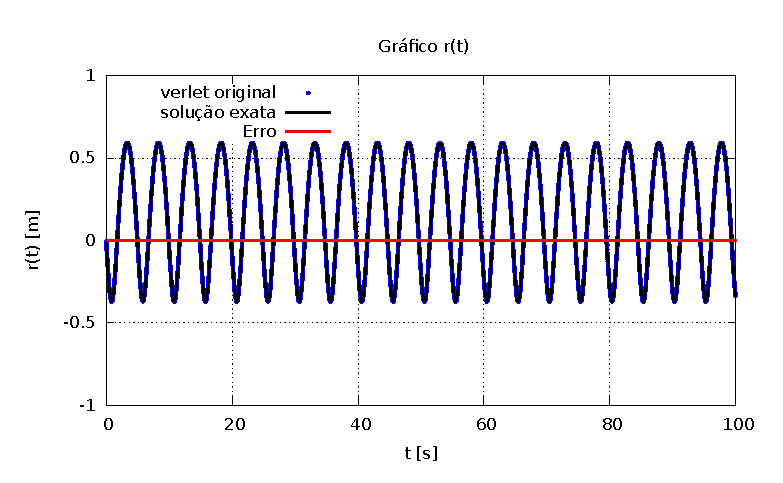
\includegraphics[scale=0.55]{ex015.eps}}\qquad 
\caption{Gráficos comparando as posições obtidas pelos métodos de verlet original, velocit verlet e Runge-Kutta com a solução exata}
\label{gra3}
\end{figure}

\newpage

Derivando a equação \ref{fun2} podemos encontrar a solução exata para a velocidade da partícula v(t), dado pela equanção \ref{fun4},
e assim também podemos comparar o quão preciso são os métodos para se calcular a velocidade da partícula e vermos qual dos métodos é mais preciso.

\begin{equation}
\centering
v(t) = \frac{-\sqrt{-2e(e+1)}sin(\sqrt{-2e}t - acos(\sqrt{e+1}))}{-1 + \sqrt{e+1}cos(\sqrt{-2e}t - acos(\sqrt{e+1}))}
\label{fun4}
\end{equation}

Na figura \ref{gra4} contrapomos respectivamente as velocidades v(t) obtidas pelos métodos de verlet original, velocity verlet e Runge Kutta com a solição exata. 

\begin{figure}[!ht]
\centering
\subfigure[Gráfico de Verlet original versus solução exata.]{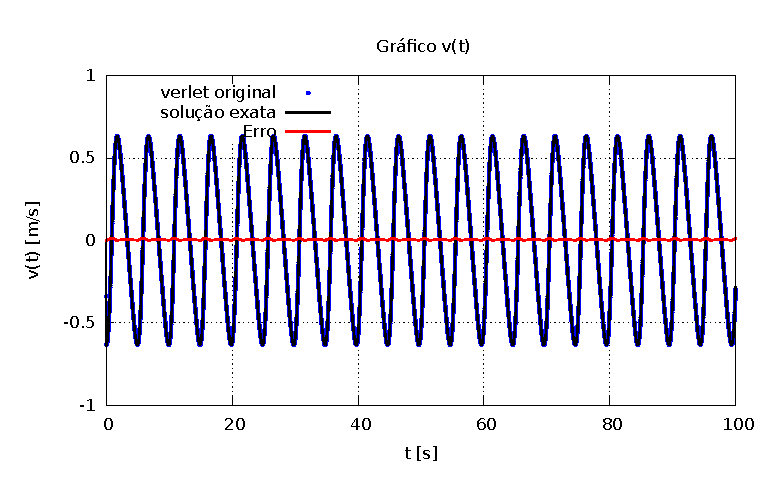
\includegraphics[scale=0.55]{ex0119.eps}}\qquad 
\subfigure[Gráfico de velocity Verlet versus solução exata.]{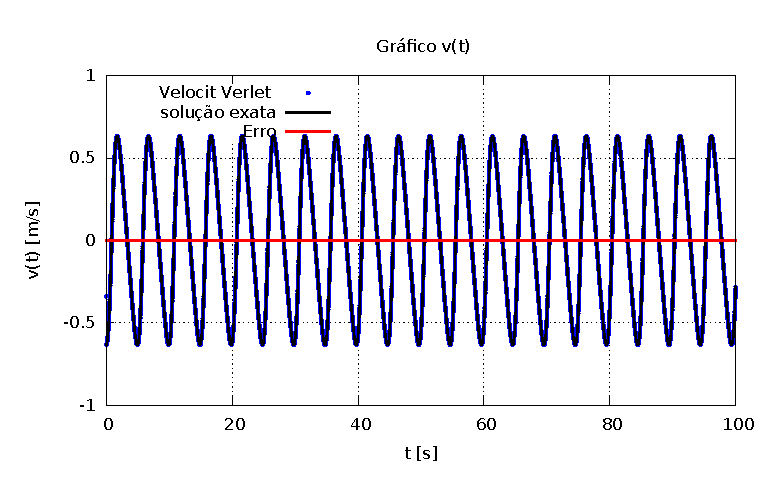
\includegraphics[scale=0.55]{ex0120.eps}}\qquad 
\subfigure[Gráfico de Runge Kutta versus solução exata.]{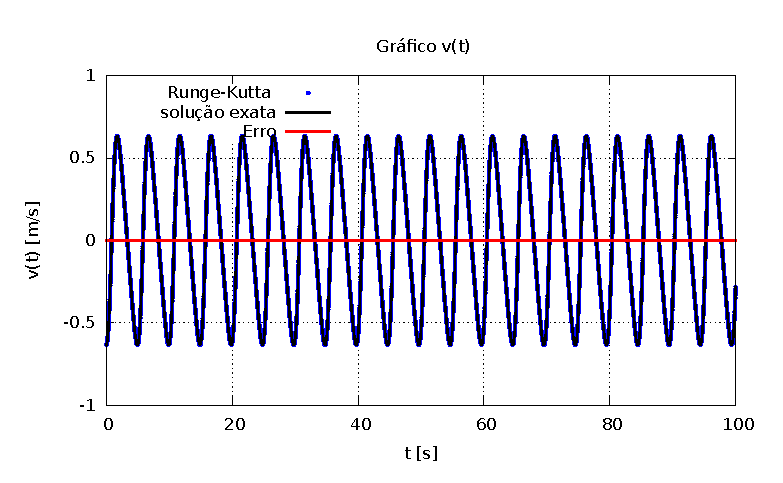
\includegraphics[scale=0.55]{ex0121.eps}}\qquad 
\caption{Gráficos comparando as velocidades obtidas pelos métodos de verlet original, velocit verlet e Runge-Kutta com a solução exata}
\label{gra4}
\end{figure}

%\newpage

Na figura \ref{gra5} tem-se dois gráficos que mostram respectivamente os erros absolutos da posição e da velocidade para os três métodos.
Observe que a solução exata para a posição e para a velocidade são dados pela equanção \ref{fun2} e \ref{fun4} respectivamente, note que
tanto para a obtenção da posição quanto para a da velocidade o método de Runge Kutta se mostrou o mais preciso, já que seu erro se mostrou 
como sendo o menor. 
\\
\begin{figure}[!ht]
\centering
\subfigure[Gráfico comparando os erros das posições obtido pelos três métodos.]{\includegraphics[scale=0.65]{ex016.eps}}\qquad 
\subfigure[Gráfico comparando os erros das velocidades obtido pelos três métodos.]{\includegraphics[scale=0.65]{ex0122.eps}}\qquad 
%\subfigure[Gráfico de Runge Kutta versus solução exata.]{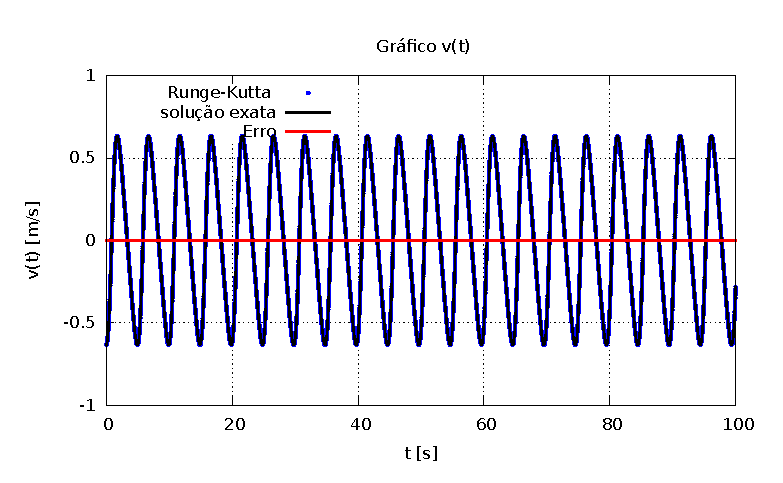
\includegraphics[scale=0.60]{ex0121.eps}}\qquad 
\caption{Gráficos dos erros absolutos para r(t) e v(t).}
\label{gra5}
\end{figure}

\newpage

\begin{quote}

\bf b- 

\end{quote}

Os cálculos de energia cinética (K), energia potencial (U) e energia mecânica (E) foram implementados nos programas $''ex01a.f90''$ e $''ex01a_Runge-kutta.f90''$, 
que por sua vez retornou dados sobre as energias da particula nos respectivos arquivos $.dat$ de cada metodo. 

O gráfico \ref{gra6} mostra as três energias da partículaobtidas pelo método $\bf Runge$ $\bf Kutta$.

\begin{figure}[!ht]
\centering
\subfigure[Energia cinética.]{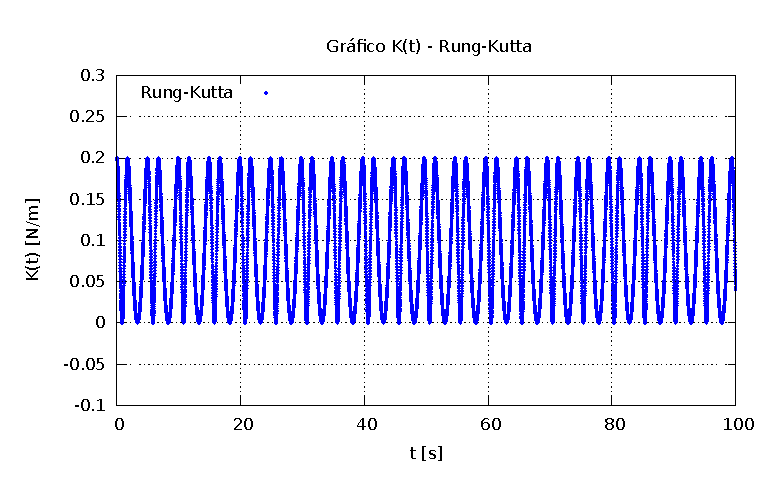
\includegraphics[scale=0.75]{ex0117.eps}}\qquad 
\subfigure[Energia potencial.]{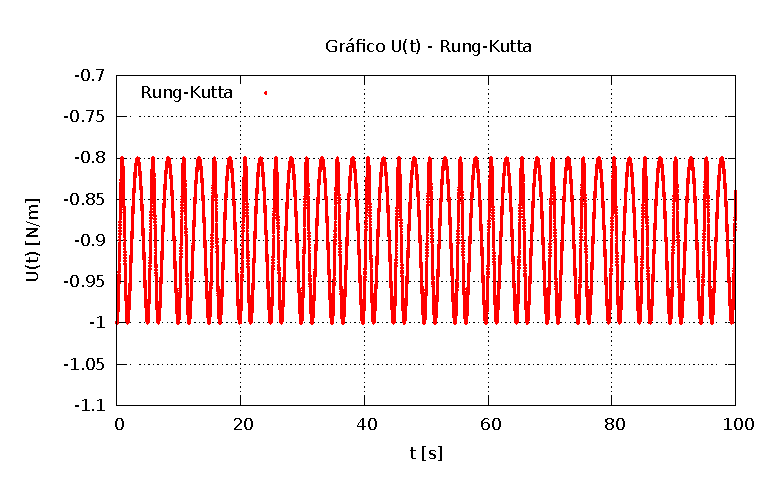
\includegraphics[scale=0.75]{ex0116.eps}}\qquad 
\subfigure[Energia mecânica.]{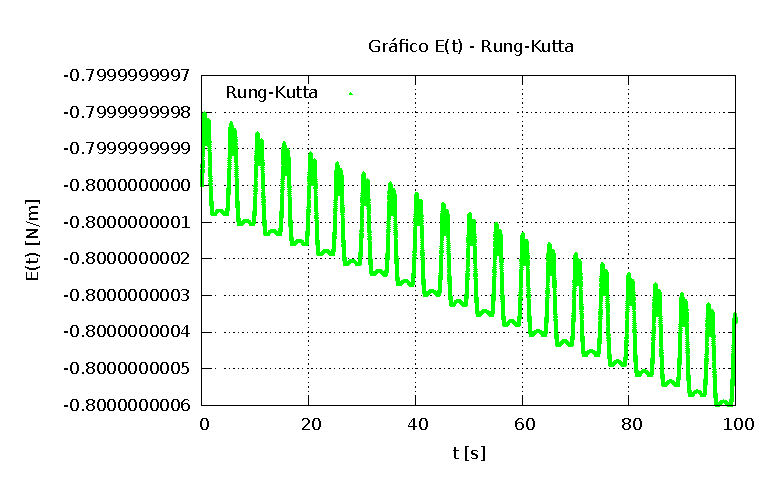
\includegraphics[scale=0.75]{ex0118.eps}}\qquad 
\caption{Gráficos das energias calculadas pelo método de Runge Kutta.}
\label{gra6}
\end{figure}

\newpage

O gráfico \ref{gra7} mostra as três energias da partícula obtidas pelo método $\bf Verlet$ $\bf original$.

\begin{figure}[!ht]
\centering
\subfigure[Energia cinética.]{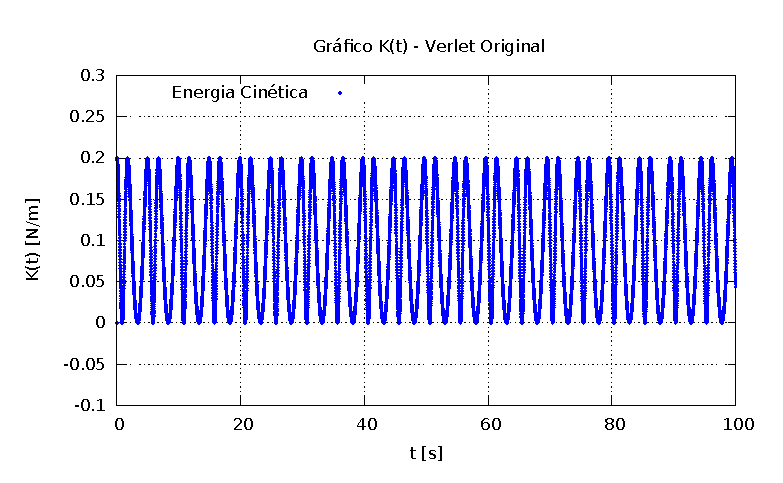
\includegraphics[scale=0.60]{ex0111.eps}}\qquad 
\subfigure[Energia potencial.]{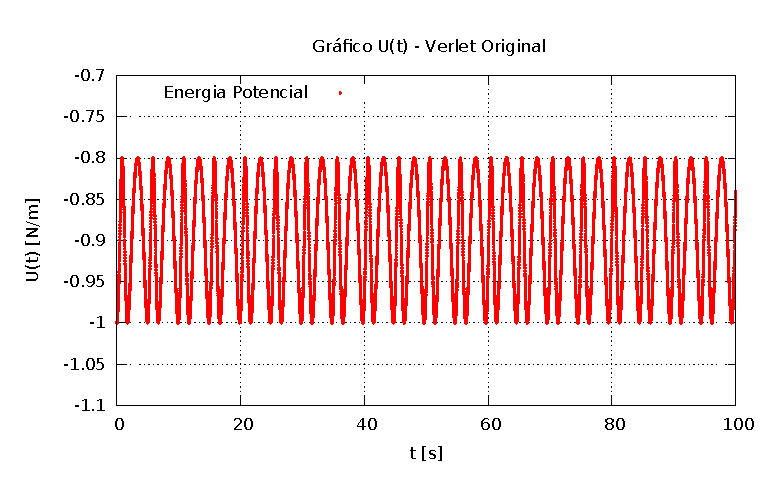
\includegraphics[scale=0.60]{ex0110.eps}}\qquad 
\subfigure[Energia mecânica.]{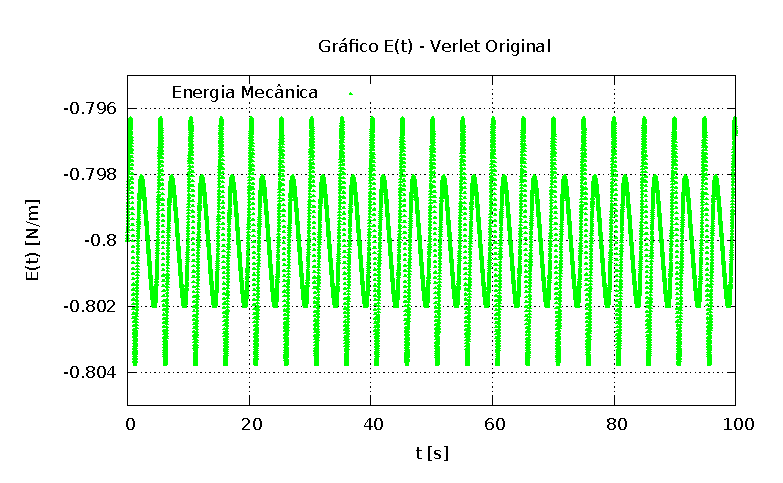
\includegraphics[scale=0.60]{ex0112.eps}}\qquad 
\caption{Gráficos das energias calculadas pelo método de Verlet original.}
\label{gra7}
\end{figure}

O gráfico \ref{gra8} mostra as três energias da partícula obtidas pelo método $\bf Velocity$ $\bf Verlet$.

\begin{figure}[!ht]
\centering
\subfigure[Energia cinética.]{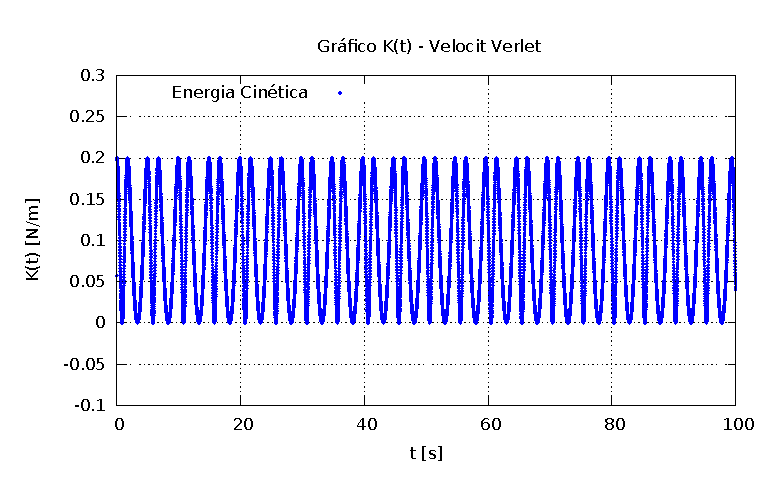
\includegraphics[scale=0.60]{ex0114.eps}}\qquad 
\subfigure[Energia potencial.]{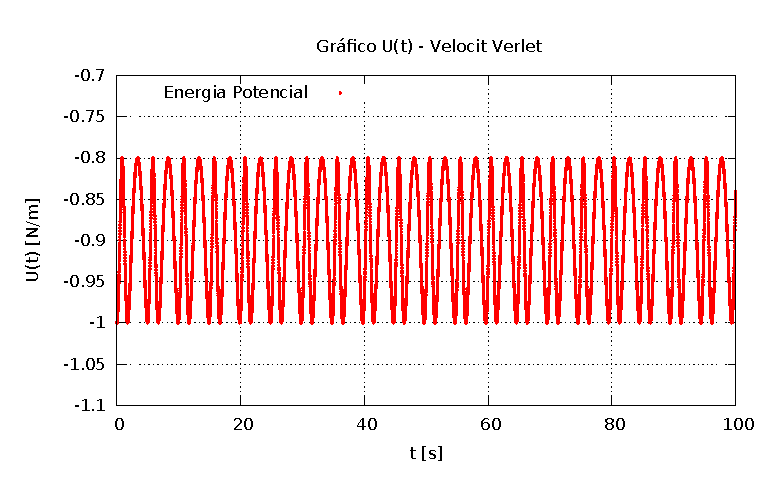
\includegraphics[scale=0.60]{ex0113.eps}}\qquad 
\subfigure[Energia mecânica.]{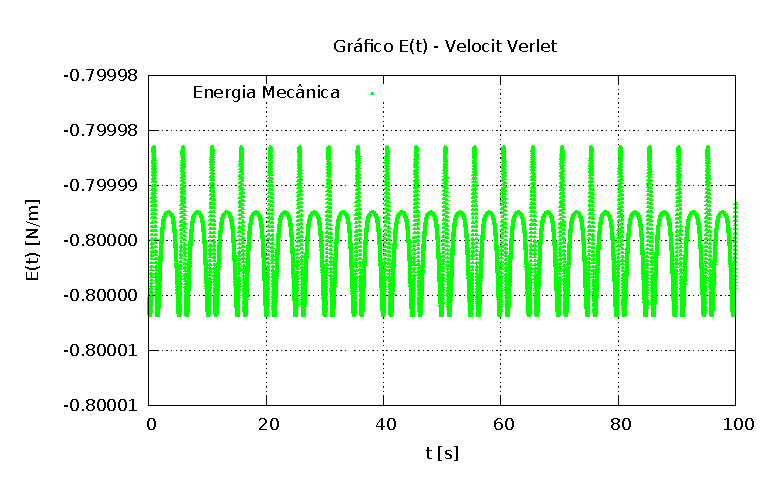
\includegraphics[scale=0.60]{ex0115.eps}}\qquad 
\caption{Gráficos das energias calculadas pelo método de Velocity Verlet.}
\label{gra8}
\end{figure}

\newpage

\begin{quote}

\bf  Exercício 2:

\end{quote}

Nesta questão foi simulado a passagem de um cometa de massa $M_{h} = 2.2 x 10^{14} Kg$ perto de uma estrela cuja massa vale 
$M_{s} = 2.0 x 10^{30} Kg$. Nos consideramos que a estrela estava parada na origem do sistema e consideramos 
também que a força que a estrela exerce no cometa seja dada pela lei da gravitação de Newton : $\Vec{F}(r) = -\frac{GM_{s}M_{h} }{r^{2}}\hat{r}$
com $G = 6.67408 x 10^{-20} Km^{3}Kg^{-1}s^{-2}$. Foi feito tudo em um único program cujo nome é $''ex02a.f90''$.

\begin{quote}

\bf  a-

\end{quote}

Nessa alternativa uma variação do método velocity Verlet foi aplicada. A aceleração tanto na componente i quanto na componente
j dependem de x(t) e y(t), então o algorítmo foi aplicado simultaneamente para o movimento em i e em j. Foram encontrados os 
valores x(t), y(t), $v_{x}(t)$ e $v_{y}(t)$ a partir disso os gráficos \ref{gra9}a  e \ref{gra9}b foram construidas. O valor da 
discretização foi escolhido de modo que ao final dos passos o cometa evolua algo próximo de 90 anos e complete sua orbita entorno da estrela, 
$\Delta t = \frac{t_{f} - t_{i}}{N}$ onde $t_{f}$ é o tempo final em segundos,$t_{i}$ é o tempo inicial em segundos e N é o número 
de intervalos. E essa discretização nos da intervalos de tempo muito grandes já que estipulei que $t_{f}$ valha 90 anos, no entanto
se aumentamos N conseguimos pegar intervalos menores porem, o computador não consegue compilar o programa que chega até a travar, por esse motivo 
escolhi um intervalo de tempo maior com um número menor de intervalos para completar a simulação, cerca de 10 mil intervalos .

\begin{figure}[!ht]
\centering
\subfigure[Trajetória do cometa.]{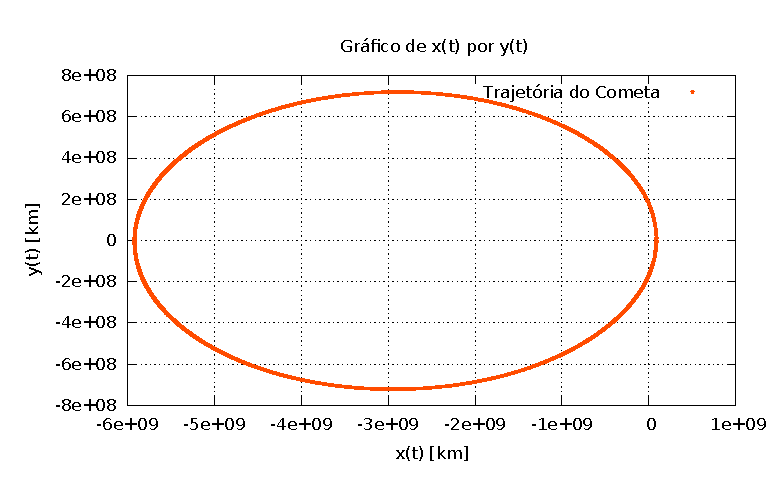
\includegraphics[scale=0.8]{ex021avelocitVerletposicoesdocometa.eps}}\qquad 
\subfigure[Velocidade do cometa.]{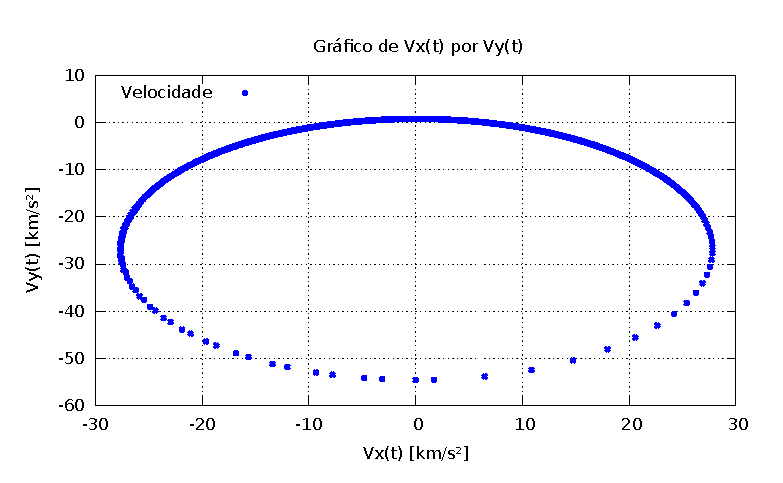
\includegraphics[scale=0.8]{ex022avelocitverletvelocidadesdocometa.eps}}\qquad 
%\subfigure[Energia mecânica.]{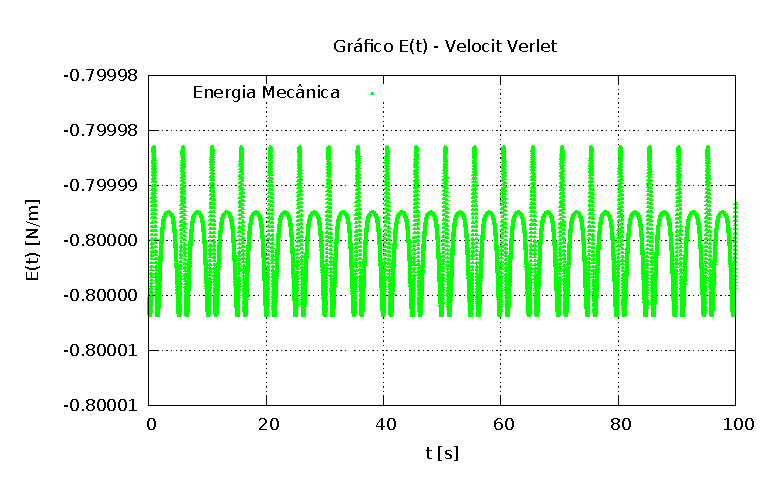
\includegraphics[scale=0.60]{ex0115.eps}}\qquad 
\caption{Gráficos da posição e da velocidade do cometa.}
\label{gra9}
\end{figure}

\newpage

\begin{quote}

\bf  b-

\end{quote}
Aqui foi pedido para que graficasse as energias potencial, cinética e mecânica e também o módulo do momento angular do cometa.
Isso esta disposto na figura \ref{gra10} que se encontra abaixo. Na figura \ref{gra11} tem-se um único gráfico contendo todas as três 
formas de energia.

\begin{figure}[!ht]
\centering
\subfigure[Energia cinética do cometa.]{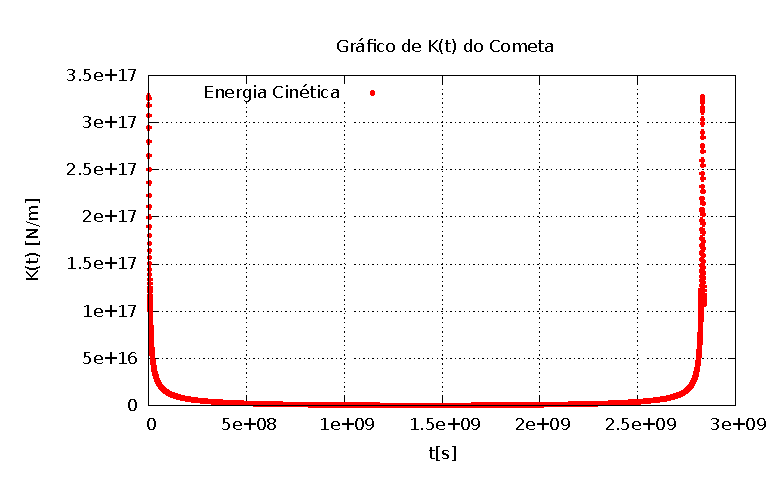
\includegraphics[scale=0.65]{ex024bEnergiaCineticadocometa.eps}}\qquad 
\subfigure[Energia potencial do cometa.]{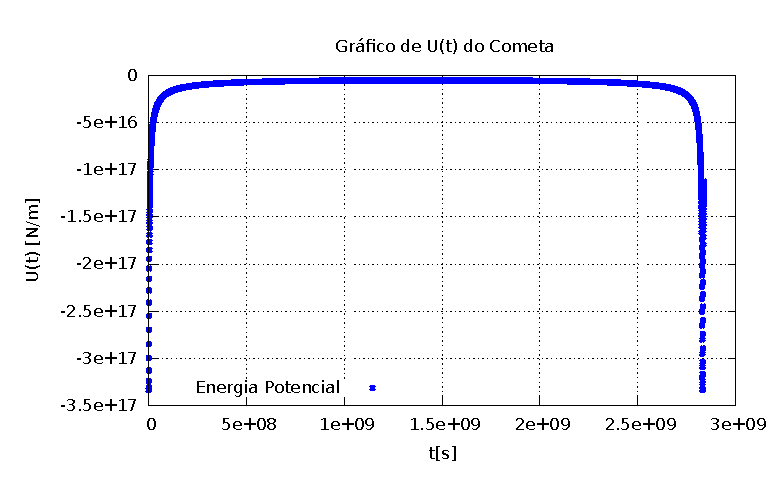
\includegraphics[scale=0.65]{ex023bEnergiaPotencialdocometa.eps}}\qquad 
\subfigure[Energia mecânica do cometa.]{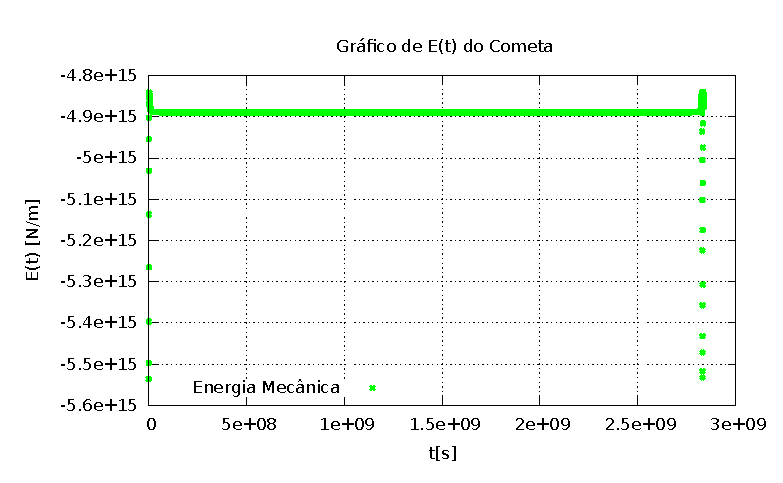
\includegraphics[scale=0.65]{ex025bEnergiaMecanicadocometa.eps}}\qquad 
\subfigure[Módulo do momento angular do cometa.]{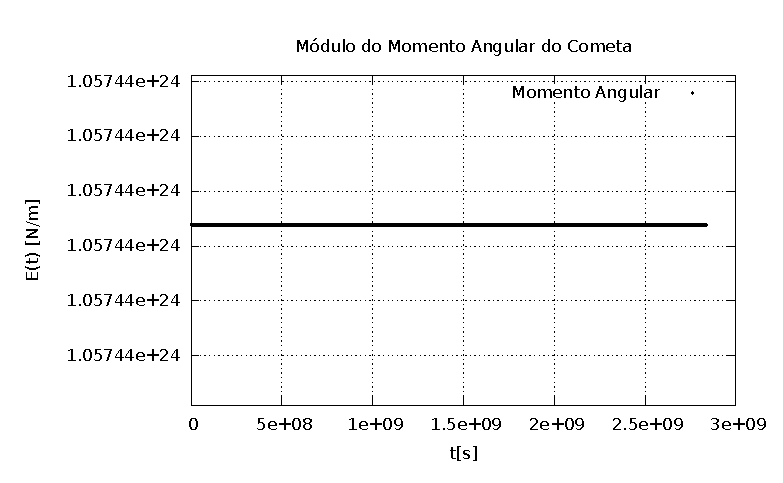
\includegraphics[scale=0.60]{ex026bMomentoAngulardocometa.eps}}\qquad 
\caption{Gráficos das energias cinética, potencial e mecânica e gráfico do módulo do momento angular.}
\label{gra10}
\end{figure}

\begin{figure}[!ht]
\centering
\includegraphics[width=0.70\textwidth]{ex027bUKE.eps}
\caption{Gráfico único contendo as energias cinética, potencial e mecânica .}
\label{gra11}
\end{figure}

\newpage

\begin{quote}

\bf  c-

\end{quote}

Sim, a trajetória deste cometa é uma órbita fechada como podemos ver na figura \ref{gra9}a, que mostra a sua trajetória ao redor da estrela.
Eu calculei o período teórico deste cometa atraves da conservação de energia e da lei dos períodos e chegei a um período teórico bem interessante.
Observe os calculos feitos estão apresentados abaixo.

Inicialmente tem-se as energias inicial e final, dadas respectivamente por \ref{Ei} e \ref{Ef}:

\begin{equation}
\centering
E_{i} = \frac{M_{h}v_{0}^{2}}{2} - \frac{GM_{h}M_{s}}{r_{0}}
\label{Ei}
\end{equation}

\begin{equation}
\centering
E_{i} = \frac{M_{h}v_{f}^{2}}{2} - \frac{GM_{h}M_{s}}{r^{,}}
\label{Ef}
\end{equation}

Sabe-se que $F = ma $ e como se trata de um cometa em orbita consta que a aceleração do cometa é uma aceleração centrípeta, assim consegue-se encontrar
$v_{f}$ de forma bem tranquila e substitui-lo na equanção \ref{Ef}, assim tem-se:

\begin{equation}
\centering
E_{i} =  - \frac{GM_{h}M_{s}}{2r^{,}}
\label{Ef1}
\end{equation}

Agora que sabe-se a equanção \ref{Ef1} foi possivel encontrar o valor do semi eixo maior da orbita do cometa, $r^{,}$. 
Ao igualar as energias final e inicial encontrei que $r^{,}$ é dado pela equação \ref{rlinha} abaixo:

\begin{equation}
\centering
r^{,} =  - \frac{GM_{h}M_{s}}{2E_{i}} \Leftrightarrow r^{,} =  - \frac{GM_{s}r_{0}}{v_{0}^{2}r_{0} - 2GM_{s} }
\label{rlinha}
\end{equation}

Assim pela lei dos periodos e pela equação \ref{rlinha} que me fornece o valor do semi eixo maior da trajetória do cometa encontrei 
um valor para o período teórico do cometa em anos, que se encontra abaixo:

\begin{equation}
\centering
T = \sqrt{\frac{4\pi^{2}r^{,3}}{GM_{s}} } \Longrightarrow T = 74.486 
\label{periodoteorico}
\end{equation}

Observe que o erro entre o período que estipulei, de 90 anos, e o período teórico encontrado é de cerca de $20\%$.

\begin{thebibliography}{99}

\bibitem{JD} J. D. Faires e R. L. Burden. Numerical Methods (3 rd ed.) 
\bibitem{FL} F. L. Moraes Barboza et al., Rev. Bras. Ens. Fís. 29 (2007) 543.
\bibitem{Metodos} C. Scherer. Metodos Computacionais da Física (2nd ed.,2010)
\bibitem{roteiro1} AULAS 21 E 22: FIS-271 - Física Computacional I
\bibitem{roteiro2} AULAS 17 E 18: FIS-271 - Física Computacional I
\end{thebibliography}
\end{document}